%
% $RCSfile: simplification.tex,v $
%
% Copyright (C) 2002-2008. Christian Heller.
%
% Permission is granted to copy, distribute and/or modify this document
% under the terms of the GNU Free Documentation License, Version 1.1 or
% any later version published by the Free Software Foundation; with no
% Invariant Sections, with no Front-Cover Texts and with no Back-Cover
% Texts. A copy of the license is included in the section entitled
% "GNU Free Documentation License".
%
% http://www.cybop.net
% - Cybernetics Oriented Programming -
%
% http://www.resmedicinae.org
% - Information in Medicine -
%
% Version: $Revision: 1.1 $ $Date: 2008-08-19 20:41:08 $ $Author: christian $
% Authors: Christian Heller <christian.heller@tuxtax.de>
%

\subsection{Simplification}
\label{simplification_heading}
\index{System as Part of Communication}
\index{Model as Part of Communication}
\index{Translator as Part of Communication}
\index{Simplified Layered Architecture}
\index{State Knowledge}
\index{Logic Knowledge}

For all three kinds of communication, there is a:

\begin{itemize}
    \item[-] \emph{System} (Human User, Database, Remote Server)
    \item[-] \emph{Model} (View, ERM, DTO)
    \item[-] \emph{Translator} (Controller/ View Assembler, Data Mapper, DTO Assembler)
\end{itemize}

\begin{figure}[ht]
    \begin{center}
        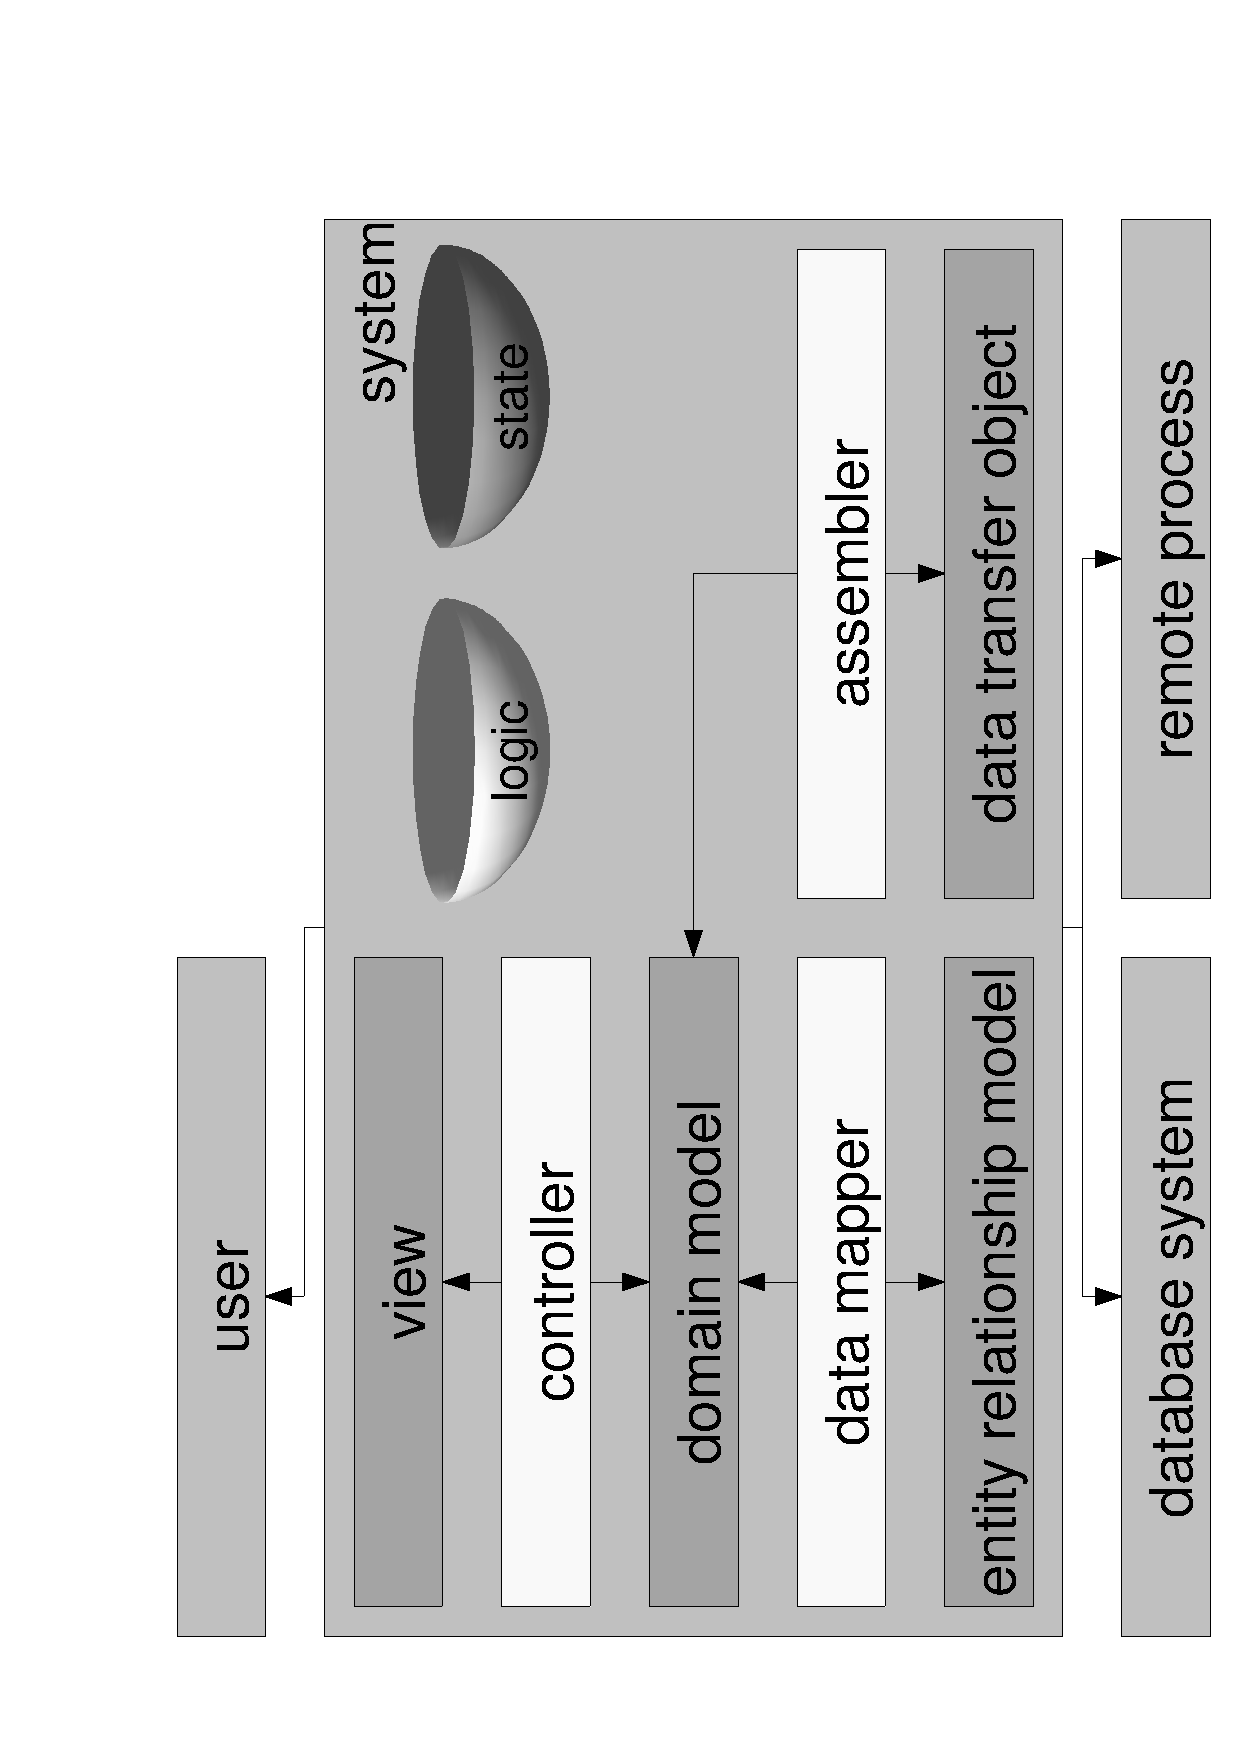
\includegraphics[scale=0.3,angle=-90]{graphic/simplification.pdf}
        \caption{Simplified Layered Architecture with State-/ Logic Knowledge}
        \label{simplification_figure}
    \end{center}
\end{figure}

All models represent certain states; all translators contain logic for
converting one state into another; all systems host their own, specific pool of
state- and logic knowledge. Realising this, a much clearer view on software
architectures can be retrieved (figure \ref{simplification_figure}).

Existing communication patterns can be merged into this common architecture.
Although these patterns suggest their very own communication paradigms, the
basic principles of interaction, as investigated on the example of transient
and persistent communication of humans in section \ref{communication_heading},
remain the same:

\begin{quote}
    An active \emph{System} (concrete process) has a mental state represented
    by passive \emph{Knowledge}. In order to exchange information with another
    system, it translates parts of its domain- into a special communication
    model which it sends to the other system. This is done by accessing its
    hardware infrastructure with \emph{input/ output} (i/o) abilities. The
    other system receives the communication model and translates it back to its
    own domain model.
\end{quote}

Because domain models differ between systems, each system needs its own
translator models. Only communication models need to be agreed upon between
systems; they need to be understood by both communication partners.
